\section{Evaluation of \acs{tfidf}}\label{sec:evaluation-tfidf}

The main obstacle to overcome was the high dimensionality of the \ac{tfidf} embeddings.
Hence, the goal of the parameter selection was to find a way to reduce the dimensionality of the vocabulary to the maximum vector dimensionality of \databaseName{}.
However, the quality of the embeddings should not decline too much.

% parameter selection
The choice of the preprocessor was investigated with regard to the goal of minimizing the vocabulary size.
Both the default and custom preprocessor were tested on a data corpus of 195 documents with regard to the vocabulary (size) and the result of preprocessing.
A visualization obtained from the comparison is given in \autoref{fig:differences-vocabularies}.
While the default preprocessor had a vocabulary size of 1641, the custom preprocessor had a size of 1906.
The custom preprocessor was chosen because it had a smaller vocabulary size.
The differences between both vocabularies were compared and visualized.
The custom vocabulary has some bigrams, which are not present in the vocabulary produced by the default preprocessor.
Initially, the idea was to have a vocabulary that consists only of unigrams.

\begin{figure}%
    \centering
    \subfloat[\centering The terms only present in the vocabulary produced by the default preprocessor.]{{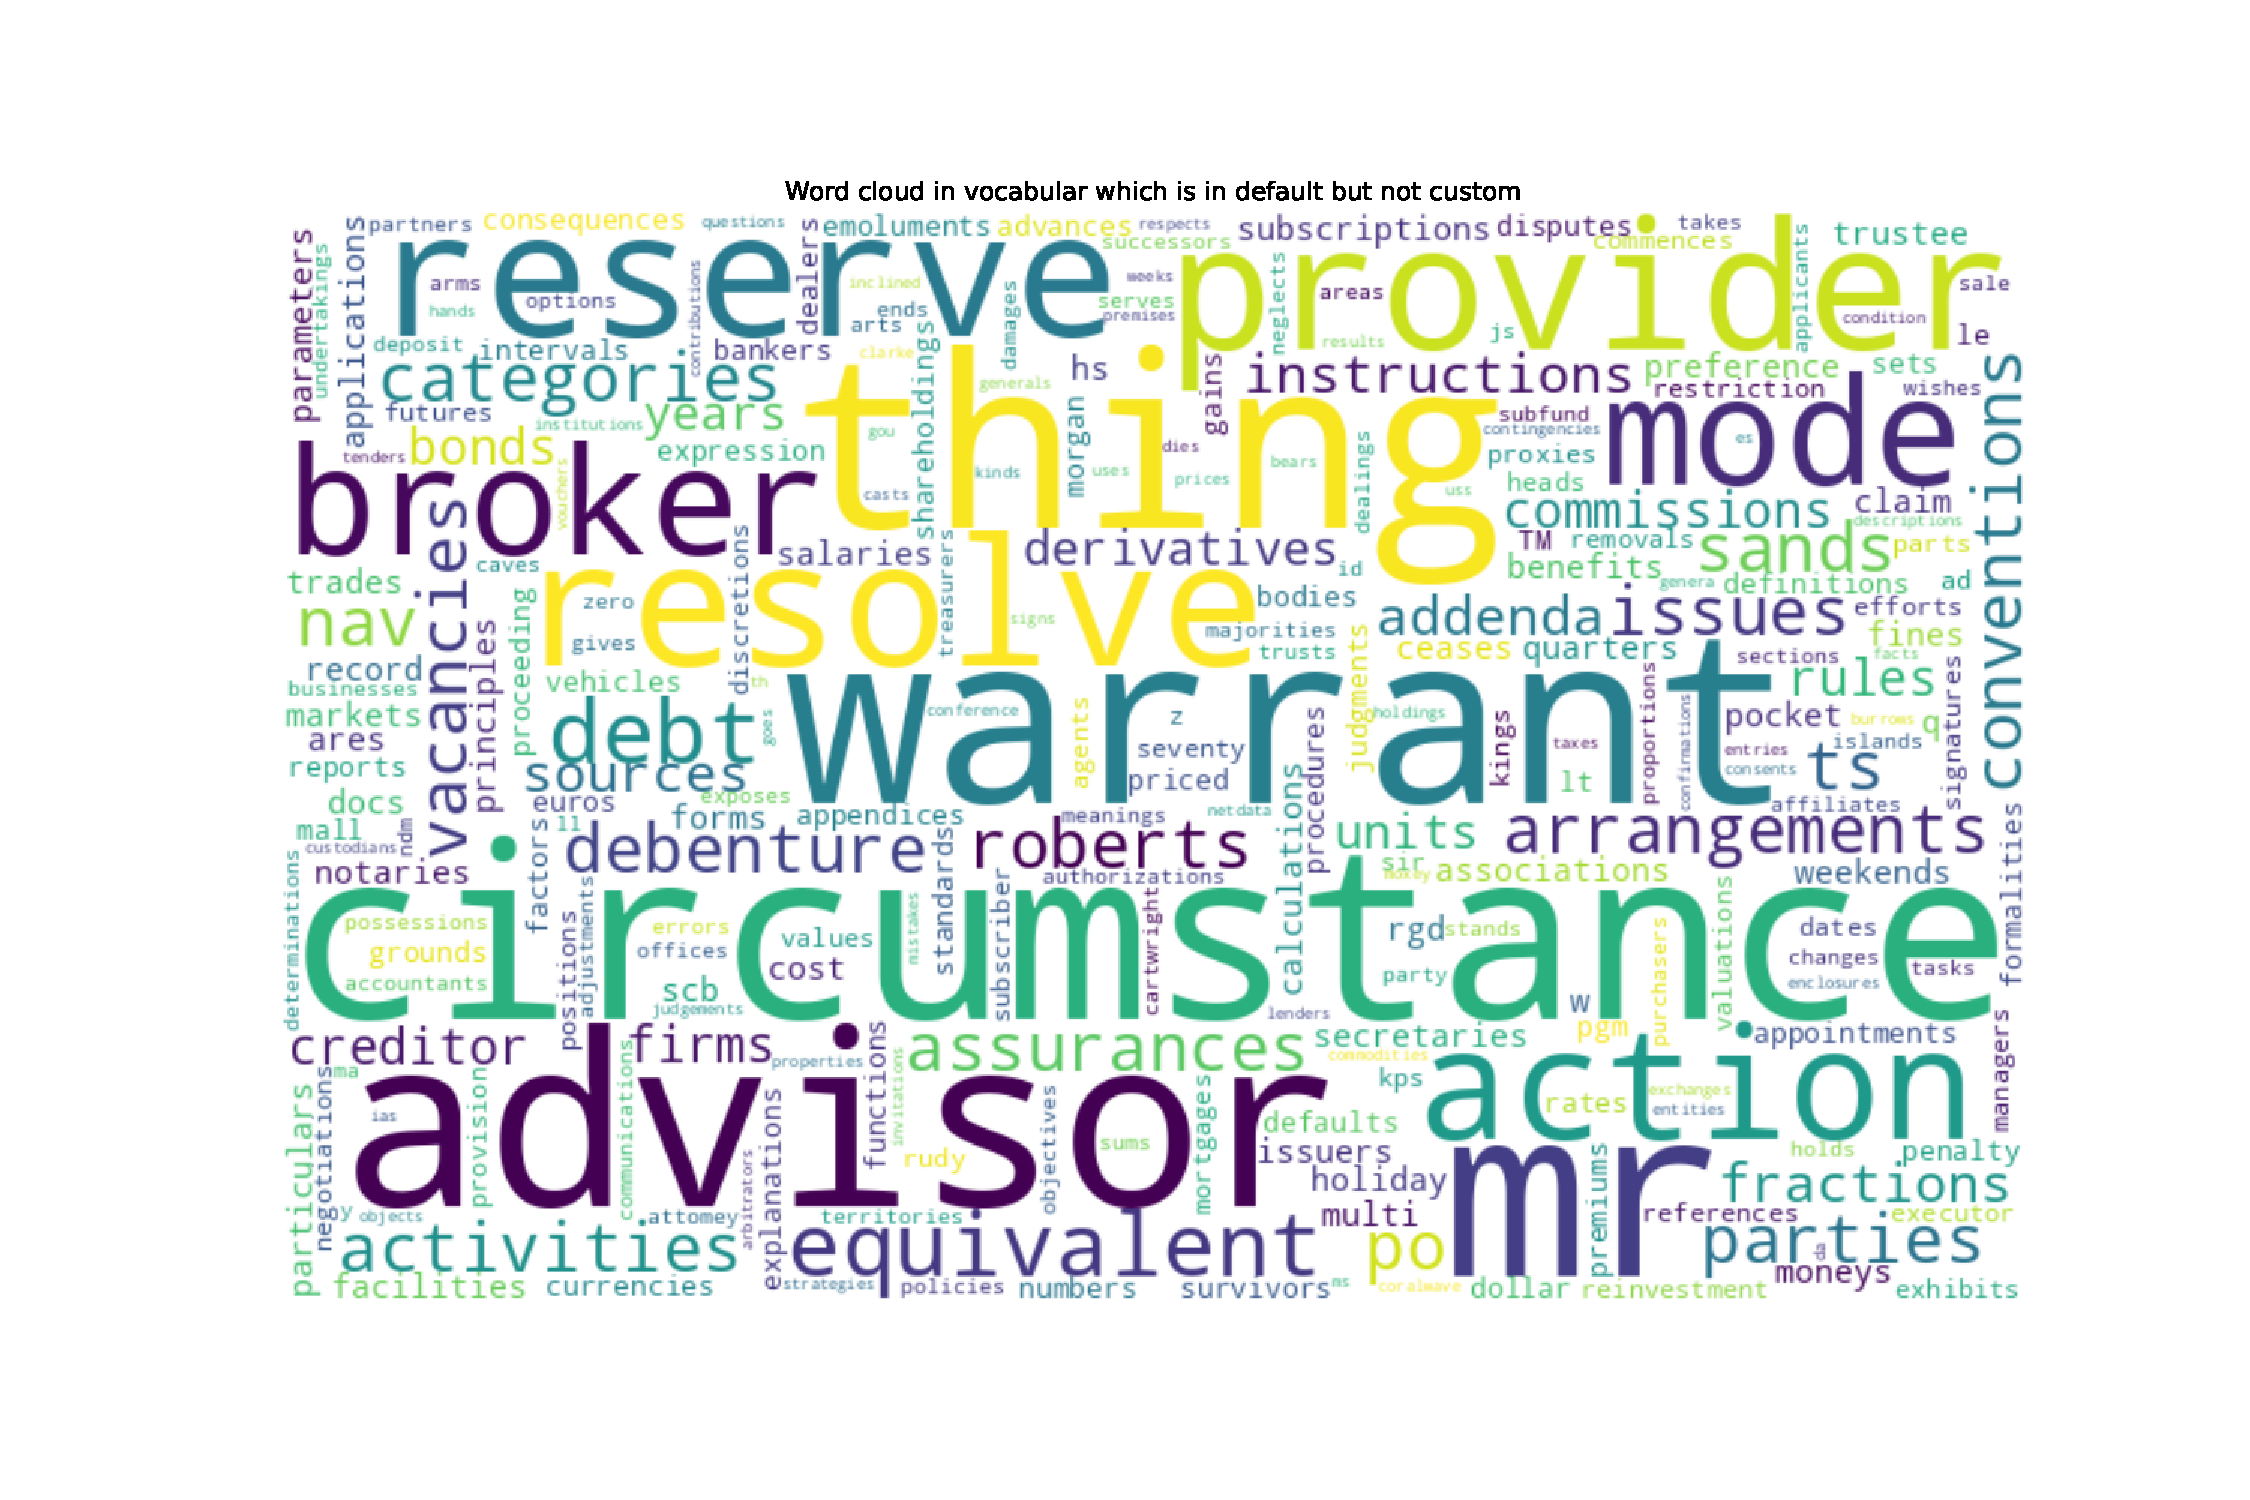
\includegraphics[width=6.5cm]{images/embeddings/tfidf/Word_cloud_in_vocabular_which_is_in_default_but_not_custom.pdf} }}%
    \qquad
    \subfloat[\centering The terms only present in the vocabulary obtained from the custom preprocessor.]{{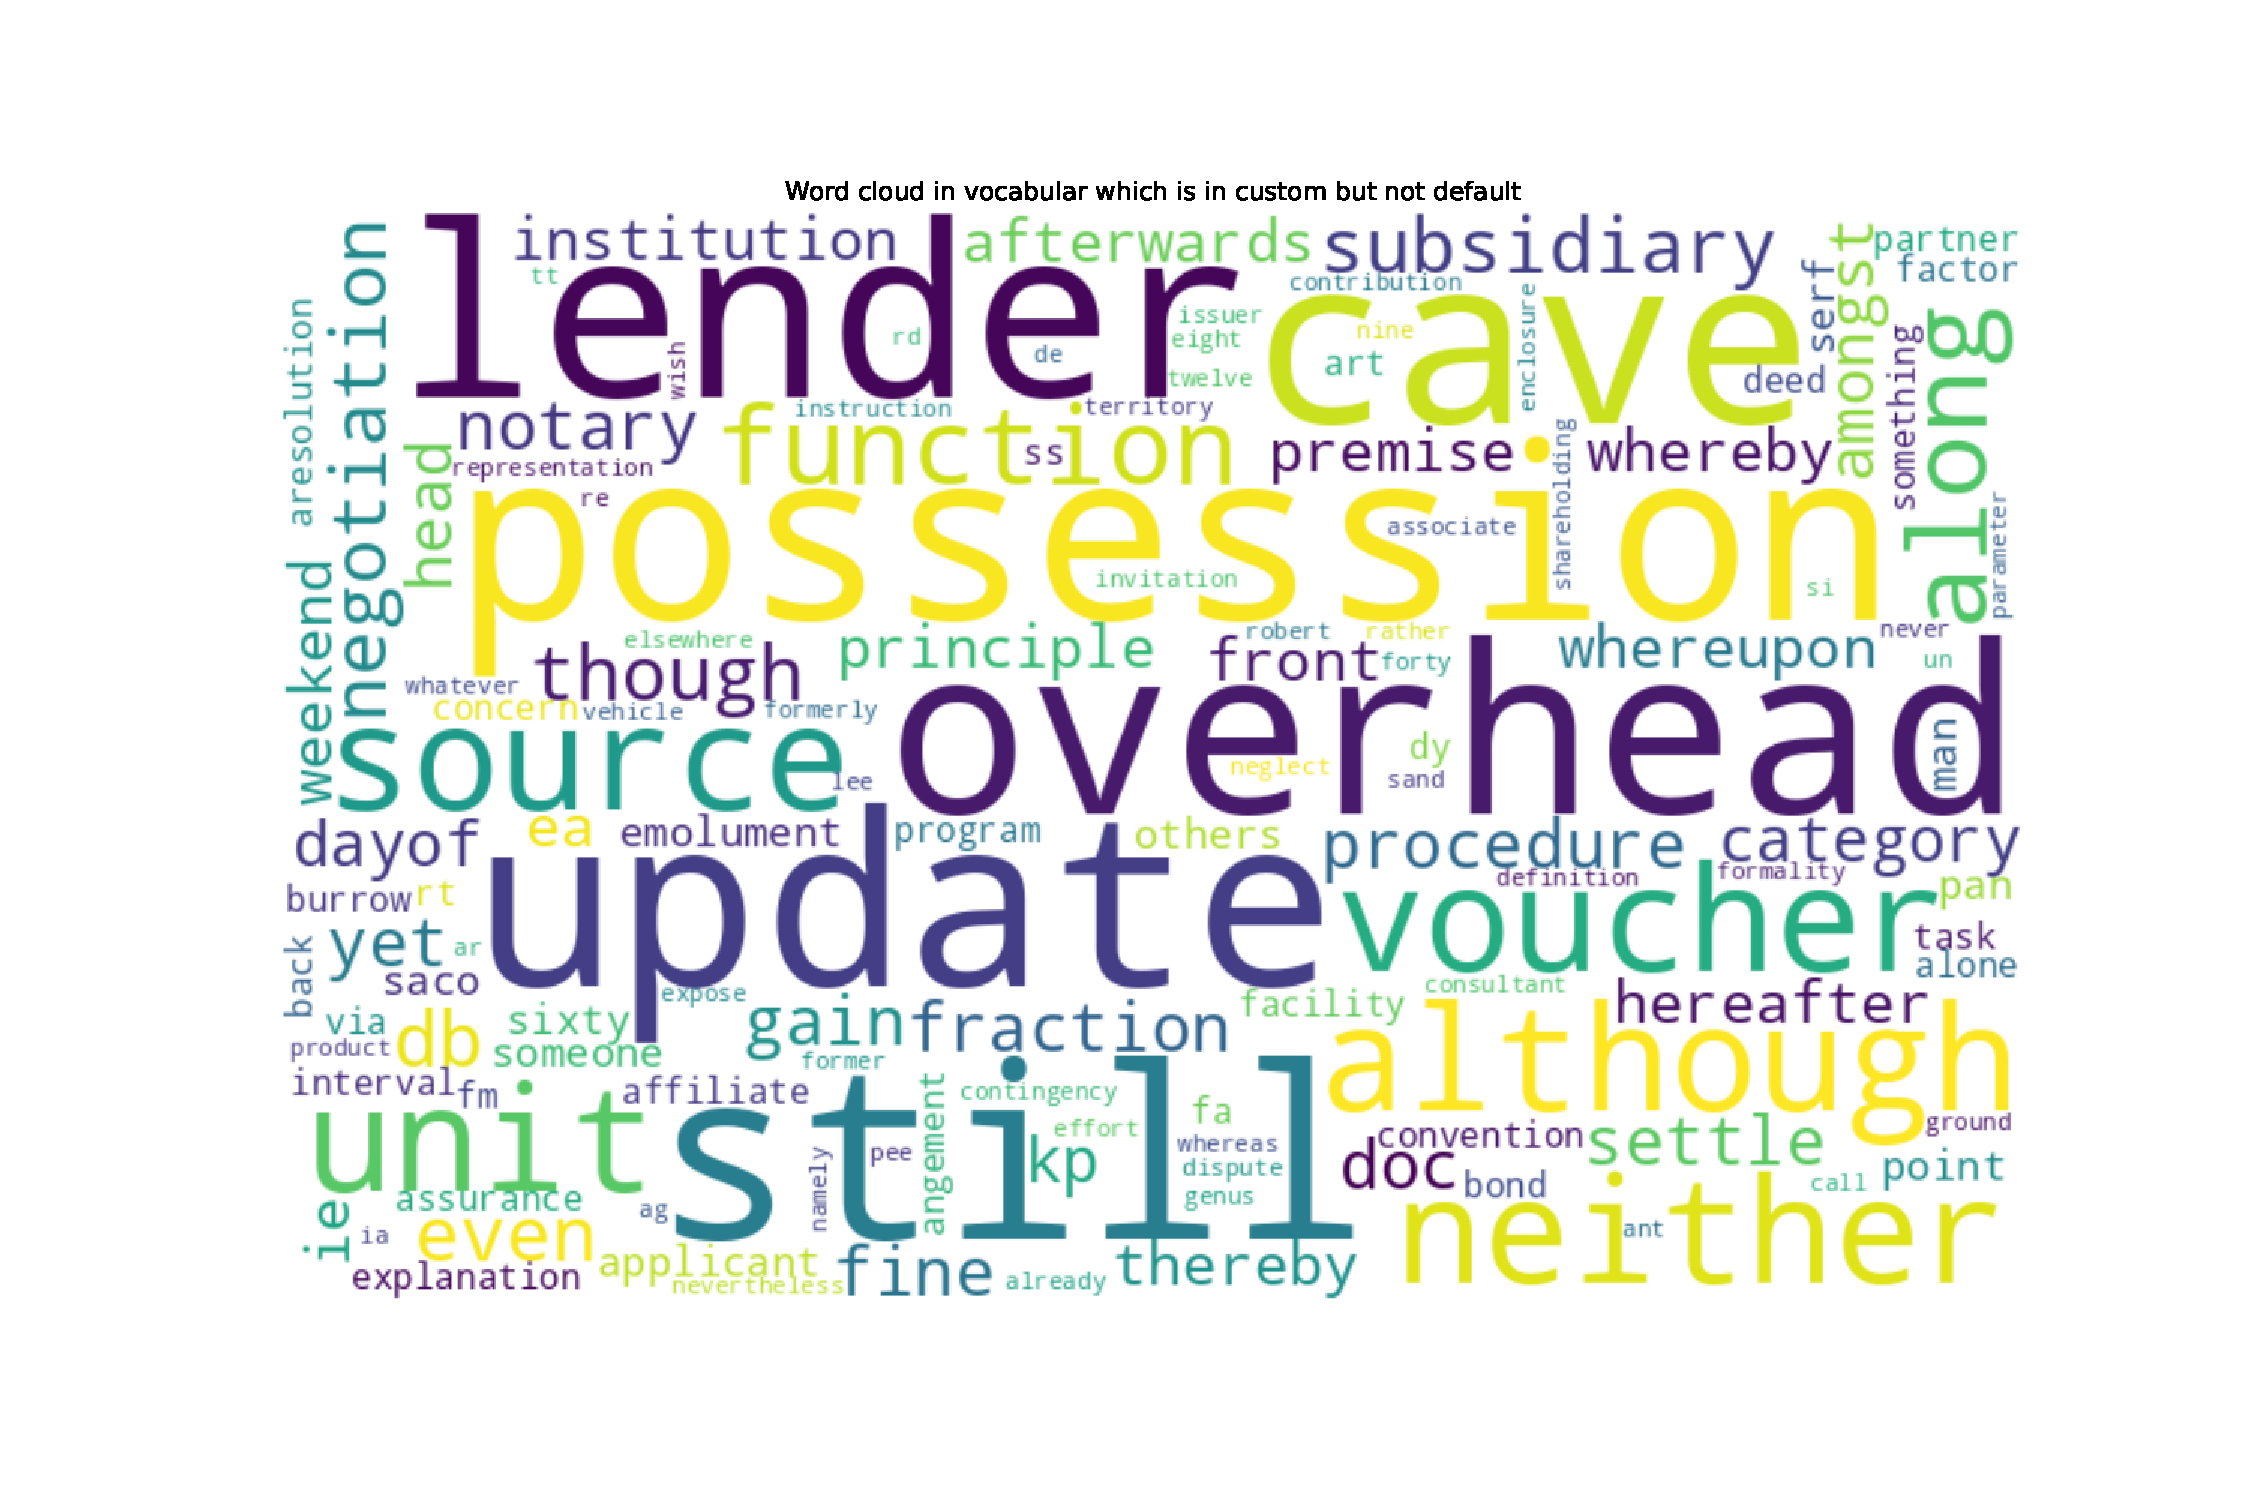
\includegraphics[width=6.5cm]{images/embeddings/tfidf/Word_cloud_in_vocabular_which_is_in_custom_but_not_default.pdf} }}%
    \caption{The WordClouds visualize which words are not shared by both vocabularies.}%
    \label{fig:differences-vocabularies}%
\end{figure}

% two fields in db
Initially, there should have been two different \ac{tfidf} models.
The first one should have been used to obtain documents which are similar to the query document.
Therefore, terms which occur only once in the corpus should have been removed from the vocabulary.
The second approach should have been used to obtain specific documents from the corpus.
Hence, the vocabulary should consist of very document-specific terms and thus, \texttt{max\_df} would have been relatively low, to omit terms that occur in many documents.
However, the restrictions imposed by the database implementation made it impossible to explore many parameter ranges.
Therefore, only one \ac{tfidf} model was used in the end, whose parameters \texttt{min\_df} and \texttt{max\_df} were set to values which kept the vocabulary and thus,
the dimensionality of the embeddings reasonably small.